%
% Presentación de TT-I.
% Planteamiento del problema.
%
% Proyecto Lovelace.
%


\section{Planteamiento del problema}

% NOTA: los títulos de las diapositivas son, aún, temporales.

\begin{frame}{Un inicio tormentoso}
  \only<1>
  {
    \begin{itemize}
      \item En la década de los 80 y 90, el comercio en línea comenzó a crecer y
        tomar importancia.
      \item Las empresas no estaban preparadas para el impacto que tuvieron y
        los fraudes relacionados con el comercio electrónico aumentaron
        rápidamente~\cite{search_security}.
        \begin{itemize}
          \item Visa y Mastercard reportaron, entre 1988 y 1998, pérdidas de 750
            millones de dólares.
        \end{itemize}
    \end{itemize}
  }

  \only<2>
  {
    \begin{figure}[H]
      \begin{center}
        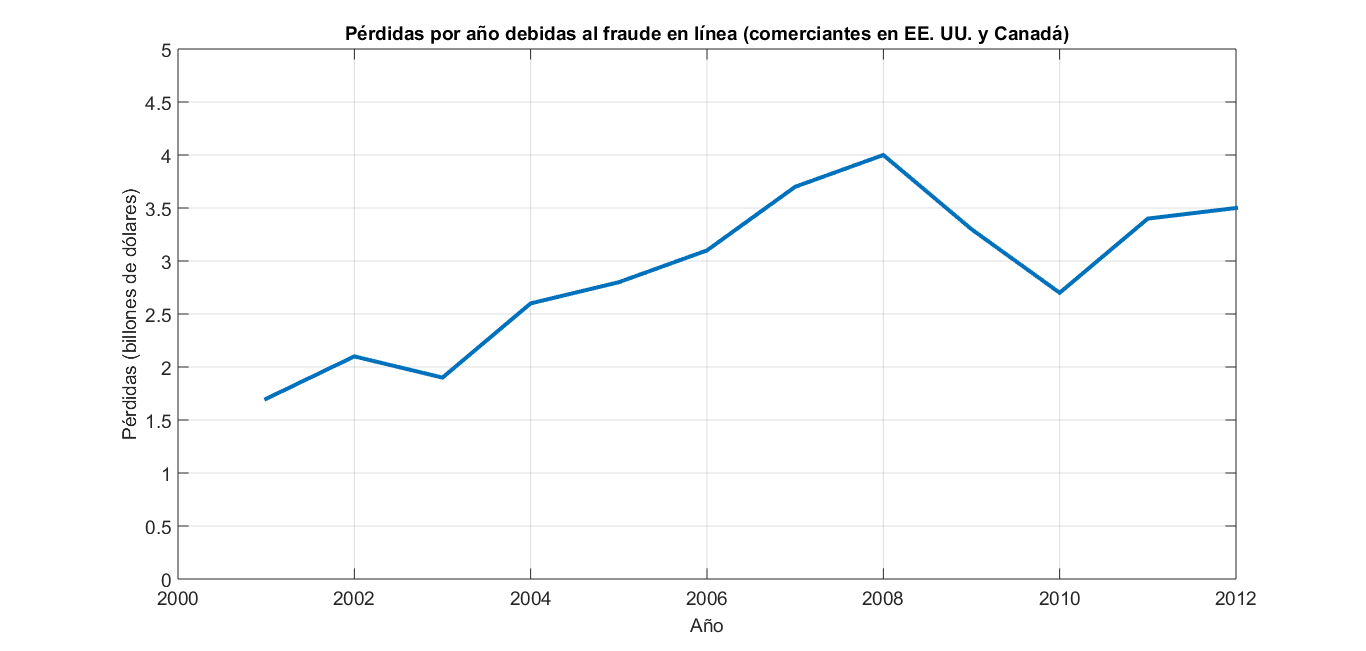
\includegraphics[width=1.0\linewidth]
          {../../diagramas_comunes/intro/perdidas_fraude}
        \caption{Pérdidas debidas al fraude en línea
          (2001-2012)~\cite{wallethub}.}
      \end{center}
    \end{figure}
  }
\end{frame}

\begin{frame}{Un estándar para gobernarlos a todos}
  % One ring to rule them all.
  \begin{itemize}
    \item A inicios del 2000, las grandes compañías emisoras de
      tarjetas\footnotemark{} comenzaron a publicar, individualmente,
      \textit{buenas prácticas} de seguridad.
      \footnotetext{
        VISA, MasterCard, American Express, entre otras.
      }
    \item Las empresas intentaron adoptar las prácticas, pero era tremendamente
      complicado y costoso.
    \item Se aliaron las compañías emisoras y, en 2004, publicaron un estándar
      unificado: PCI-DSS\footnotemark~\cite{pci_dss}.
      \footnotetext{
        Payment Card Industry - Data Security Standard
      }
      \begin{itemize}
        \item Se hizo obligatorio para quienes realizasen más de 20K
          transaccciones al año.
        \item Tiene un gran número de requerimientos (y subrequerimientos), por
          lo que es difícil de satisfacer.
      \end{itemize}
  \end{itemize}

  % \note
  % {
  %   Al mencionar el primer punto hay que poner ejemplos de estas compañías:
  %   Visa, Master Card, American Express, etc.
  % }

\end{frame}

\begin{frame}{Cambio de estrategia}
  \begin{itemize}
    \item Hasta ahora, el enfoque era proteger los datos sensibles donde sea
      que se encuentren y por donde sea que transiten.
    \item Surge un nuevo enfoque: cambiar la información valiosa, por
      \textit{valores representativos} (tokens); es decir, la tokenización
      de la información.
    \item En 2011, el PCI-SSC\footnotemark{} publicó las primeras guías para los
      procesos de tokenización~\cite{pci_tokens}.
      \begin{itemize}
        \item Aunque indica lo que debe satisfacer el sistema tokenizador,
          no dice cómo generar los tokens.
      \end{itemize}
  \end{itemize}
  \footnotetext{
    Payment Card Industry - Security Standards Council
  }
\end{frame}

\begin{frame}{Pero ¿por qué?}
  A pesar de ser una práctica extendida, la tokenización sigue estando
  rodeada de desinformación y desconfianza.
  \begin{itemize}
    \item Se busca combatir la desinformación al estudiar e implementar cinco
      algoritmos tokenizadores, compararlos y mostrar los resultados.
    \item Hacer notar que la criptografía y la tokenización no están peleadas;
      pues la tokenización puede verse como una aplicación de la criptografía.
  \end{itemize}
\end{frame}
